\documentclass{article}
\usepackage[top=2cm, left=1.5cm, right=1.5cm, bottom=2cm]{geometry}
\usepackage{graphicx}
\usepackage{wrapfig}
\usepackage{amsmath}
\usepackage{tcolorbox}
\graphicspath{{./img/}}
\setlength{\parindent}{0pt}

\title{Systems of Linear Equations}
\date{16-Nov-2023}

\begin{document}
\maketitle
\section{What is a system of linear Equations?}

A linear equation in the variables $x_1,x_2,\dots, x_n $ is an equation that can be written in the form $ax_1,ax_2,\dots, ax_n = b$ where $b$ and the coefficients $ a_1, a_2,\dots, a_n $ an are real or complex numbers, the subscript $n$ may be any positive integer. In real-life problems, n might be 50 or 5000, or even larger. The equations \newline $$4x_1 - 5x_2 + 2 = x_1$$ $$x_2 = 2(\sqrt{6} - x_1) + x_3$$ \newline

Because they can be rearranged algebraically as:
$$3x_1-5_x2 = -2$$
$$2x_1 + x_2 - x_3 = 2 \sqrt{6}$$ 
The equations $$4x_1 - 5x_2 = x_1x_2$$ $$x_2 = 2\sqrt{x_1} - 6$$\newline are not linear because of the presence of $x_1, x_2$ in the first equation and $\sqrt{x1}$ in the second. A system of linear equations (or a linear system) is a collection of one or more linear equations involving the same variables. $$2x_1 - x_2 + 1.5x_3 = 8$$ $$x_1 \hspace{10 mm} - 4x_3 = -7$$\\
A solution of the system is a list $(s_1,s_2,\dots, s_n)$ of numbers that makes each equation a true statement when the values $(s_1,s_2,\dots, s_n)$ are substituted for $(x_1,x_2,\dots, x_n)$, respectively.
The set of all possible solutions is called the solution set of the linear system. Two linear systems are called equivalent if they have the same solution set.\newline

\subsection{Two Variables}

\begin{wrapfigure}{l}{0.3\textwidth} 
    \centering
    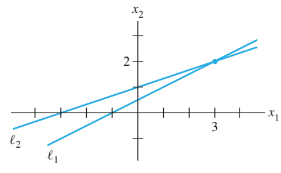
\includegraphics[width=0.3\textwidth]{image.png}
    \caption{1 Solution}
\end{wrapfigure}
Finding the solution set of a system of two linear equations in two variables is easy because it amounts to finding the intersection of two lines. Example: $$x_1 - 2x_2 = -1$$
$$-x_1 + 3x_2 = 3$$\newline
The graphs of these equations are lines, which we denote by $l_1$ and $l_2$. A pair of numbers $(x_1, x2_)$ satisfies both equations in the system if and only if the point $(x_1, x2_)$ lies on both $l_1$ and $l_2$. In the system above, the solution is the single point (3, 2).\pagebreak

\begin{wrapfigure}{r}{0.3\textwidth} 
    \centering
    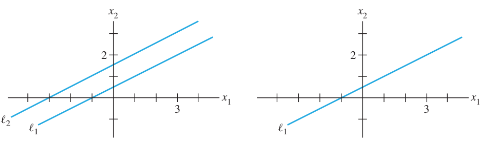
\includegraphics[width=0.3\textwidth]{image1.png}
    \caption{No solutions}
\end{wrapfigure}

Two lines need not intersect in a single point, they could be parallel, or they could coincide and hence “intersect” at every point on the line. For the graph 1, we dont have a solution, and for the graph 2, we have infinitely solutions. Thereforea system of linear equations has:

\begin{itemize}
    \item[-] No solution 
    \item[-] Exactly one solution
    \item[-] Infinitely many solutions \newline
\end{itemize} 

A system is said to be inconsistent if has no solution and a system is consistent if it has either 1 solution or infinitely solutions. If we are workin with 3 variables, we are looking a point that lies in the planes i.e.

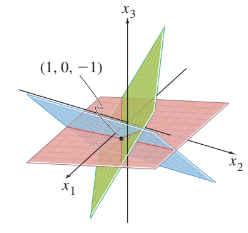
\includegraphics{image2.png}

In other dimensions we also have the same cases, there is no solution, there is one or infinite. In a third dimension the cases would look like this: 

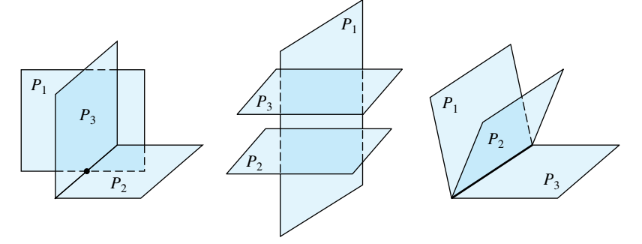
\includegraphics{image4.png}

\pagebreak

\subsection{Matrix Notation}

The essential information of a linear system can be recorded compactly in a rectangular array called a matrix.

\begin{align*}
    \quad & x_1 - 2x_2 + \phantom{0} x_3 = 0 \\
    \quad & \phantom{1x_1+} 2x_2 -8x_3 = 8\\
    \quad & 5x_1 \phantom{+2x_2} -5x_3 = 10
\end{align*}

Coefficient Matrix: the coefficients of each variable aligned in columns

$$\begin{bmatrix}
    1&-2&1\\
    0&2&-8\\
    5&0&-5
\end{bmatrix}$$

Augmented Matrix: coefficient matrix with an added column containing the constants from the right sides of the equation. \newline

$$\left[\begin{array}{ccc|c}
    1&-2&1&0 \\
    0&2&-8&8 \\
    5&0&-5&10 \pagebreak
\end{array}\right]$$

\subsection {Solving a Linear System}

The basic strategy is to replace one system with an equivalent system (one with the same solution set) that is easier to solve. Three elementary rows operations are used to simplify a linear system. 

\begin{itemize}
    \item[-] (Replacement) Replace one row by the sum of itself and a multiple of another row
    \item[-] (Interchange) Interchange two rows.
    \item[-] (Scaling) Multiply all entries in a row by a nonzero constant.
\end{itemize}

Example

\begin{alignat*}{2}
    \begin{matrix}
        x_1 - 2x_2 + x_3 &= 0\\
        \phantom{x_1+} 2x_2 -8x_3 &= 8\\
        5x_1 \phantom{+2x_2} -5x_3 &= 10
    \end{matrix}
    & \hspace{ 4em}%
    \begin{bmatrix}
        1 & -2 & 1 & 0\\
        0 & 2 & -8 & 8\\
        5 & 0 & -5 & 10
    \end{bmatrix}
\end{alignat*}

. \newline

Keep $x_1$ in the first equation and eliminate it from de other equations. To do so, add -5 time equation 1 to equation 3.

\begin{alignat*}{2}
    \begin{matrix} 
        \begin{split}
            -5\cdot\text{[equation 1]}\\
            +\text{[equation 3]}\\
            \hline
            \text{[new equation 3]} \\ 
        \end{split}
    \end{matrix}
    & \hspace{ 4em}%
    \begin{matrix} 
        \begin{split}
            -5x_1 + 10x_2 - 5x_3 &= 0\\
            5x_1 \phantom{+10x_2} - 5x_3 &=10\\
            \hline
            \phantom{-5x_1+} 10x_2 - 10x_3 &=10 \\ 
        \end{split}
    \end{matrix}
\end{alignat*}

\noindent Now in order to obtain 1 as the coefficient for $x_2$ in equation 2, multiply equation 2 by 1/2. With the 2 previous operations we obtain:

\begin{equation*}
    \begin{bmatrix}
        1 & -2 & 1 & 0\\
        0 & 1 & -4 & 4\\
        0 & 10 & -10 & 10
    \end{bmatrix}
\end{equation*}

\noindent Use $x_2$ in equation 2 to eliminate the $10x_2$ in equation 3.

\begin{alignat*}{2}
    \begin{matrix} 
        \begin{split}
            -10\cdot\text{[equation 2]}\\
            +\text{[equation 3]}\\
            \hline
            \text{[new equation 3]}
        \end{split}
    \end{matrix}
    & \hspace{ 4em}%
    \begin{matrix} 
        \begin{split}
            -10x_2 + 40x_3 &= -40\\
            10x_2 - 10x_3 &= 10\\
            \hline
            \phantom{-10x_2+}30x_3 &= -30
        \end{split}
    \end{matrix}
\end{alignat*}

\noindent  The result of this calculation written in place of the previous thir equation is:

\begin{equation*}
    \begin{bmatrix}
        1 & -2 & 1 & 0\\
        0 & 1 & -4 & 4\\
        0 & 0 & 30 & -30
    \end{bmatrix}
\end{equation*}

\noindent Now, multiply equation 3 by 1/30 to obtain 1 as the coefficient for $x_3$:

\begin{alignat*}{2}
    \begin{matrix} 
        \begin{split}
            x_1 - 2x_2 + x_3 &= 0\\
            \phantom{x_1-2} x_2 - 4x_3 &= 4\\
            \hline
            \phantom{ x_1 - 2x_2 +} x_3 &= -1
        \end{split}
    \end{matrix}
    & \hspace{ 4em}%
    \begin{bmatrix}
        1 & -2 & 1 & 0\\
        0 & 1 & -4 & 4\\
        0 & 0 & 1 & -1
    \end{bmatrix}
\end{alignat*}

\noindent Use $x_3$ in equation 3 to eliminate the $-4x_3$ and $x_3$ in equations 1 and 2.

\begin{alignat*}{2}
    \begin{matrix} 
        \begin{split}
            -1\cdot\text{[equation 3]}\\
            +\text{[equation 1]}\\
            \hline
            \text{[new equation 1]}
        \end{split}
    \end{matrix}
    & \hspace{ 4em}%
    \begin{matrix}
        \begin{split}
            4\cdot\text{[equation 3]}\\
            +\text{[equation 2]}\\
            \hline
            \text{[new equation 2]}
        \end{split}
    \end{matrix}
\end{alignat*}

\noindent Obtainig:

\begin{equation*}
    \begin{bmatrix}
        1 & -2 & 0 & 1\\
        0 & 1 & 0 & 0\\
        0 & 0 & 1 & -1
    \end{bmatrix}
\end{equation*}

\noindent Move back to equation 2 and use it to eliminate the $-2x_2$ above it, since there is now no arithmetic involving $x_3$ terms.

\begin{alignat*}{2}
    \begin{matrix} 
        \begin{split}
            2\cdot\text{[equation 2]}\\
            +\text{[equation 1]}\\
            \hline
            \text{[new equation 1]}
        \end{split}
    \end{matrix}
    & \hspace{ 4em}%
    \begin{bmatrix}
        1 & 0 & 0 & \phantom{-}1\\
        0 & 1 & 0 & \phantom{-}0\\
        0 & 0 & 1 & -1
    \end{bmatrix}
\end{alignat*}

\noindent Finally, we get the values for each $x$:

$$\begin{matrix} 
    \begin{aligned}
        x_1\phantom{x_2+x_3} &= 1\\
        \phantom{x_1} x_2 \phantom{+x_3} &= 0\\
        \phantom{x_1+} \phantom{2x_2 +} x_3 &= -1\\
    \end{aligned}
\end{matrix}$$

.\newline

It is important to note that row operations are reversible. Any solution of the original system remains a solution of the new system. Conversely, since the original system can be produced via row operations on the new system, each solution of the new system is also a solution of the original system.

\subsection{Existence and Uniqueness}

Is the system consistent; that is, does at least one solution exist?
If a solution exists, is it the only one; that is, is the solution unique?

Example : Determine if the following matrix is consistent: 

$$\begin{matrix} 
    \begin{aligned}
        \phantom{x_1} x_2 - 4x_3 &= 8\\
        2x_1 - 3x_2 + 2x_3 &= 1\\
        4x_1 - 8x_1 + 12x_3 &= 1
    \end{aligned}
\end{matrix}$$

\noindent After some matrx operations we obtain the triangular form, which is:

$$\begin{matrix} 
    \begin{aligned}
        2x_1 - 3x_2 - 2x_3 &= 1\\
        \phantom{x_1+} x_2 - 4x_3 &= 8\\
        \phantom{x_1 + x_2 +} 0 &= 15
    \end{aligned}
\end{matrix}$$

\noindent The equation 3 is a short form of $0x_1 + 0x_2 + 0x_3 = 15$. This system has a built-in contradiction. There are no values of $x_1$, $x_2$, $x_3$ that satify because the equation $0=15$ is never true. Therefore the system is \textbf{inconsistent} (i.e. has no solution).

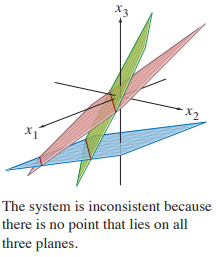
\includegraphics{image3.png}

\subsection{Row Reduction and Echelon Forms}

This section refines into a row reduction algorithm that will enable us to analyze any system of linear equations. By using only the first part of the algorithm, we will be able to answer the fundamental existence and uniqueness questions posed in the previous Section.\newline

The algorithm applies to any matrix, whether or not the matrix is viewed as an augmented matrix for a linear system. So the first part of this section concerns an arbitrary rectangular matrix and begins by introducing two important classes of matrices that include the “triangular” matrices. In the definitions that follow, a nonzero row or column in a matrix means a row or column that contains at least one nonzero entry; a leading entry of a row refers to the leftmost nonzero entry (in a nonzero row).\newline

A  rectangular matrix is in echelon form (or row echelon form) if it has the following three properties:

\begin{tcolorbox}[colback=blue!10!white,colframe=blue!60!black,title=Echelon Form Properties]
    \begin{itemize}
        \item[1.] All nonzero rows are above any rows of all zeros.
        \item[2.] Each leading entry of a row is in a column to the right of the leading entry of the row above it.
        \item[3.] All entries in a column below a leading entry are zeros.
    \end{itemize}
    If a matrix in echelon form satisfies the following additional conditions, then it is in reduced echelon form (or reduced row echelon form):
    \begin{itemize}
        \item[4.] The leading entry in each nonzero row is 1.
        \item[5.] Each leading 1 is the only nonzero entry in its column.
    \end{itemize}
\end{tcolorbox}

\begin{large}
    Example Echelon Form
\end{large}

The leading entries (.) may have any nonzero value; the starred entries (*) may have any value (including zero).

\begin{alignat*}{2}
    \begin{bmatrix}
        .&*&*&*\\
        0&.&*&*\\
        0&0&0&0\\
        0&0&0&0
    \end{bmatrix}
    & \hspace{ 4em}%
    \begin{bmatrix}
        0&.&*&*&*&*&*&*&*&*\\
        0&0&0&.&*&*&*&*&*&*\\
        0&0&0&0&.&*&*&*&*&*\\
        0&0&0&0&0&.&*&*&*&*\\
        0&0&0&0&0&0&0&0&.&*
    \end{bmatrix}
\end{alignat*}

\pagebreak

\begin{large}
    Example Reduced Echelon Form
\end{large}

The leading entries are 1's and there are 0's below and above each leading 1.

\begin{alignat*}{2}
    \begin{bmatrix}
        1&0&*&*\\
        0&1&*&*\\
        0&0&0&0\\
        0&0&0&0
    \end{bmatrix}
    & \hspace{ 4em}%
    \begin{bmatrix}
        0&1&*&0&0&0&*&*&0&*\\
        0&0&0&1&0&0&*&*&0&*\\
        0&0&0&0&1&0&*&*&0&*\\
        0&0&0&0&0&1&*&*&0&*\\
        0&0&0&0&0&0&0&0&1&*
    \end{bmatrix}
\end{alignat*}

\noindent Any nonzero matrix may be row reduced into more than one matrix in echelon form, using different sequences of row operations. However, the reduced echelon form one obtains from a matrix is unique.

\begin{tcolorbox}[colback=blue!10!white,colframe=blue!60!black,title=Uniqueness of Row Reduced Echelon Form ]
    Each matrix is row equivalent to one and only one reduced echelon matrix.
\end{tcolorbox}
    
If a matrix A is row equivalent to an echelon matrix U, we call U an echelon form (or row echelon form) of A; if U is in reduced echelon form, we call U the reduced echelon form of A.

\begin{tcolorbox}[colback=blue!10!white,colframe=blue!60!black,title=Pivot Positions]
    A pivot position in a matrix A is a location in A that corresponds to a leading 1 in the reduced echelon form of A, a pivot column is a column of A that contains a pivot position.
\end{tcolorbox}

\subsubsection*{Row Reduction Algorithm}

The algorithm that follows consists of four steps, and it produces a matrix in echelon form. A fifth step produces a matrix in reduced echelon form. \newline

\begin{large}
    Example:
\end{large}
Apply elementary row operations to transform the following matrix first into echelon form and then into reduced echelon form: 

\begin{equation*}
    \begin{bmatrix}
        0&\phantom{+}3&-6&\phantom{-}6&4&-5\\
        3&-7&\phantom{-}8&-5&8&\phantom{-}9\\
        3&-9&12&-9&6&15
    \end{bmatrix}
\end{equation*}


\begin{tcolorbox}[colback=green!20!white,colframe=green!80!black,title=Step 1]
    Begin with the leftmost nonzero column. This is a pivot column. The pivot position is at the top.
    \end{tcolorbox}

\begin{tcolorbox}[colback=green!20!white,colframe=green!80!black,title=Step 2]
    Select a nonzero entry in the pivot column as a pivot. If necessary, interchange rows to move this entry into the pivot position.
\end{tcolorbox}

Interchange rows 1 and 3. (We could have interchanged rows 1 and 2 instead)

\begin{equation*}
    \begin{bmatrix}
        3&-9&12&-9&6&15\\
        3&-7&\phantom{-}8&-5&8&\phantom{-}9\\
        0&\phantom{+}3&-6&\phantom{-}6&4&-5\\
    \end{bmatrix}
\end{equation*}

\pagebreak
\begin{tcolorbox}[colback=green!20!white,colframe=green!80!black,title=Step 3]
    Use row replacement operations to create zeros in all positions below thw pivot.
\end{tcolorbox}
Add -1 times row 1 to row 2.

\begin{equation*}
    \begin{bmatrix}
        3&-9&12&-9&6&15\\
        0&\phantom{-}2&-4&4&2&-6\\
        0&\phantom{+}3&-6&6&4&-5\\
    \end{bmatrix}
\end{equation*}

\begin{tcolorbox}[colback=green!20!white,colframe=green!80!black,title=Step 4]
    Ignore the row containing the pivot position and all rows, if any, above it. Apply steps 1-3 to the submatrix that remains. Repeat the process until there are no more nonzero rows to modify.
\end{tcolorbox}

Step 1 shws that column 2 is the next pivot column, for step 2, select as a pivot the top entry in that column. \newline For step 3, we could insert an optional step of dividing the top row of the submatrix by the pivot. Instead we add -3/2 times the top row below. Which produces:

\begin{equation*}
    \begin{bmatrix}
        3&-9&12&-9&6&15\\
        0&\phantom{-}2&-4&\phantom{-}4&2&-6\\
        0&\phantom{+}0&\phantom{-}0&\phantom{-}0&1&\phantom{-}4
    \end{bmatrix}
\end{equation*}

Steps 1-3 require no work for this submatrix, and we have reached an echelon form of the full matrix. If we want the reduced echelon form, we perform one more step

\begin{tcolorbox}[colback=green!20!white,colframe=green!80!black,title=Step 5]
    Beginning with the rightmost pivot and working upward and to the left, create zeros above each pivot. If a pivot is not 1, make it 1 by a scaling operation.
\end{tcolorbox}

The rightmost pivot is in row 3. Create zeros above it, adding suitable multiples of row 3 to rows 2 and 1. \newline The combination of steps 1-4 is called the forward phase of the row reduction algorithm. Step 5, which produces the unique reduced echelon form, is called the backward phase.

\end{document}